
\chapter{Equilibres  et  potentiels  thermodynamiques}

\section{Potentiels thermodynamiques}

Soit un système thermodyamique isochore et isotherme, situé dans un thermostat calorifugé 

\begin{figure}[H]
\centering
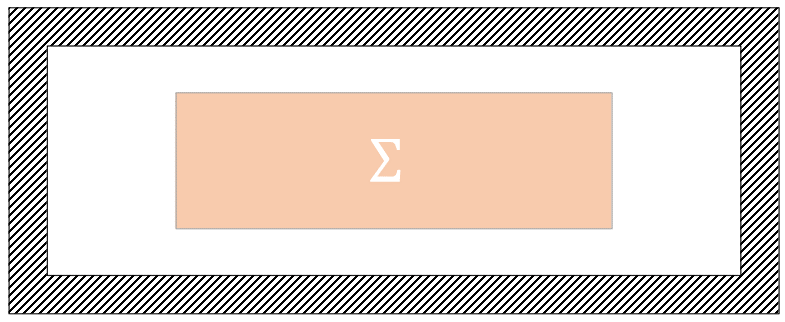
\includegraphics[scale=0.4]{C4F1.PNG}
\caption{Système thermodynamique $\Sigma$ dans un thermostat}
\end{figure}

Dans cette situation, on a un volume constant donc pas de travail, on en déduit :
$$dU_{\Sigma}=\delta Q \textrm{ et } dS_{th}=\frac{\delta Q_{th}}{T}$$
On a donc
$$\delta Q_{\Sigma}+\delta Q_{th}=0 \textrm{ et } dS=-\frac{\delta Q}{T}$$
Or, on a notre variation élémentaire d'entropie telle que
$$dS=\delta S_e+\delta S_c$$
Notre chaleur échangée étant nulle, puisqu'on a un système adiabatique, on obtient
$$dS=\delta S_c \geq 0$$
On en déduit ainsi
\begin{equation*}
\left \{ \begin{array}{l} dS = dS_{th}+dS_{\Sigma} \geq 0 \\dS_{\Sigma} - \frac{\delta Q}{T}=dS_{\Sigma} - \frac{dU_{\Sigma}}{T}\geq 0 \end{array} \right. \Rightarrow dU_{\Sigma}-TdS_{\Sigma}\geq 0
\end{equation*}

On pose alors $dF=dU_{\Sigma}-TdS_{\Sigma}$

\begin{definition}[Energie libre]
Soit le potentiel thermodynamique appelé énrgie libre et noté $F$ tel que 
\begin{equation}
F=U-TS
\end{equation}
Par définition, le critère de stabilité de l'équilibre sera donné tel que $F$ minimal et $S$ maximal.
\end{definition}

\begin{proposition}{Différentielle de l'énergie libre.  }
On définira la différentielle de $F$ telle que 
\begin{align}
F&=U-TS\notag\\
\Rightarrow dF &= dU-TdS-SdT\notag\\
\Leftrightarrow dF &= \delta Q + \delta W -TdS -SdT\notag\\
\Leftrightarrow \bf{dF }&\bf{=-PdV -SdT}
\end{align}

\end{proposition}

Ainis, lorsque l'on a une transformation spontannée istotherme, $F$ diminue et l'état d'équilibre correspond à un minimum d'énergie libre.

\begin{definition}[Enthalpie libre]
Soit le potentiel thermodynamique appelé énergie libre et noté $G$ tel que 
\begin{equation}
G=H-TS
\end{equation}
Et dont la différentielle s'exprime telle que \footnote{Démonstration effectuée au chapitre précédent}
\begin{equation}
dG=VdP-SdT
\end{equation}
On notera que de façon générale $dG\leq 0$
\end{definition}

\section{Travail maximal récupérable}

Pour un système monotherme, soit un système dont les températures initale et finale sont égales, on a 
$$\Delta S = S_B-S_A \geq \frac{Q}{T} \Rightarrow Q \leq T\Delta $$
Or, on a 
$$W=\Delta U - Q \Leftrightarrow \Delta U - W = Q \leq T\Delta S$$
A partir de la définition de l'énergie libre, on a 
$$\Delta F = \Delta U - T \Delta S$$
On en déduit donc le théroème suivant 
\begin{theorem}[Energie libre d'une transformation monotherme]
Lors d'une transformation monotherme, le travail $W$ récupérable de l'extérieur de notre système est supérieur ou égal à la variation d'énergie libre $\Delta F$ de notre système. Ainsi, on a 

\begin{equation}
\Delta F \leq W
\end{equation}

Dans le cadre d'une transformation réversible, notre inégalité se transformera en égalité.

\end{theorem}

\begin{example}[Compression dans un récipient aux parois dithermes]
On effectue la dillatation d'un gaz dans un récipient aux parois diathermes, c'est-à-dire dans le cadre d'une transformation monotherme. On posera $V_b=10~V_a$.

\begin{figure}[H]
\centering
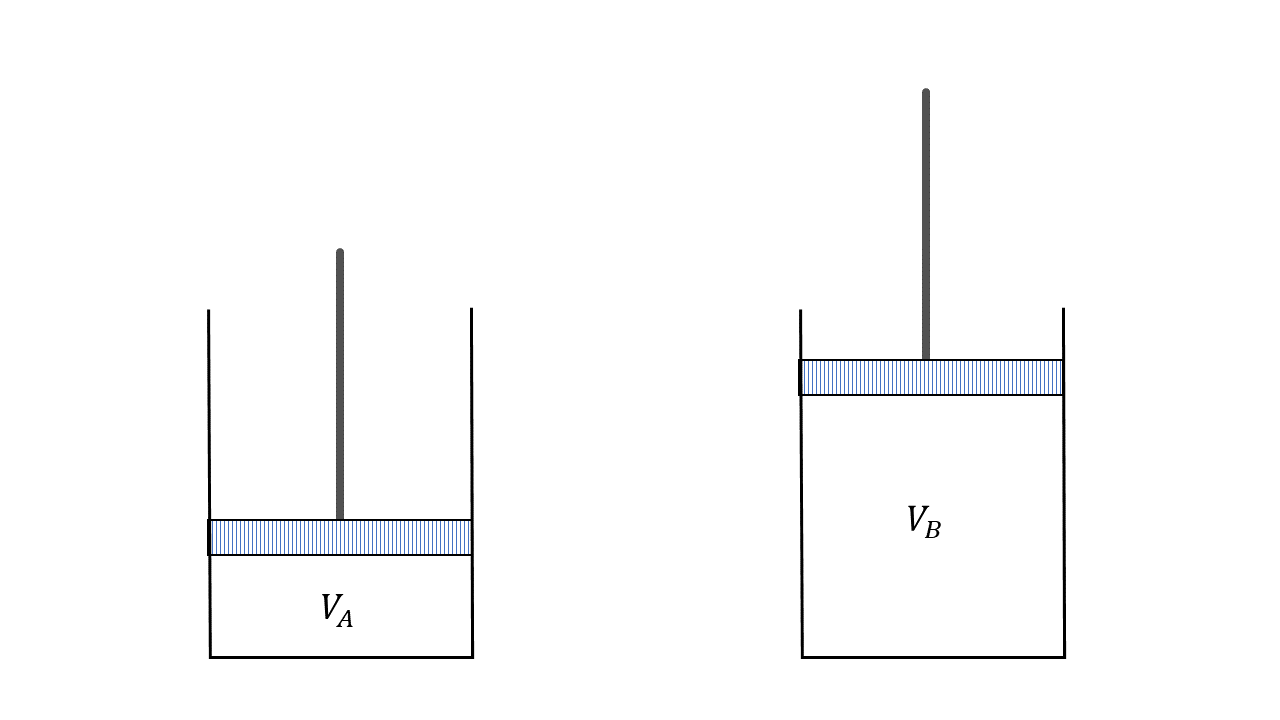
\includegraphics[scale=0.35]{C4F2.PNG}
\caption{Dillatation d'un gaz dans des conditions monothermes}
\end{figure}

On a 
$$dF = -SdT-PdV=-PdV = nRT\frac{dV}{V}$$

Donc
$$\Delta F = -nRT\ln\frac{V_B}{V_A}$$

On pose notre réacion comme réversible, on a donc 
$$\Delta F = W$$
$$W = -8,314 \times 298 \times \ln 10 = 5,7~kJ$$
\end{example}

\section{Equilibre chimique}

Soit la réaction chimique 
$$aA_{(g)}+cC_{(g)}\rightleftharpoons lL_{(g)}+rR_{(g)}$$

On définit le sens 1 allant de la gauche vers la droite et le sens 2, opposé au sens 1. On a ainsi :

$$\Delta_rG_m=\Delta_rG_m^0+RT\ln M$$

Où $M$ est le monôme des activité, tel que pour une réactio  exclusivement en phase gazeuse

$$M=\prod \left ( \frac{P_i}{P_0}\right ) ^{\nu_i}$$

Où $\nu_i$ sont les coefficients stoechiométriques de nos produits et réactifs chimiques. Ici, on a donc 

$$M=\frac{P(R)^r.P(L)^l}{¨(A)â.P(C)^c}P_0^{(a+c-r-l)}$$

Notre réaction s'effectue, on a donc $P(A)$ et $P(C)$ qui diminuent, quand $P(R)$ et $P(L)$ qui augmentent. Notre monôme $M$ augmente alors lui aussiet donc $\Delta_rG_m$ aussi. A l'équilibre, on a un équilibre de composition, soit
$$\Delta_rG_m = G_{prod}-G_{react}=0$$
Notre réaction est donc stoppée, ce qui implique que 
$$\Delta_rG_m = 0 \Leftrightarrow \Delta_rG_m^0 +RT \ln M_{eq}=0$$

\begin{definition}[Variation d'enthalpie libre à l'équilibre]
A l'équilibre, la varaition d'enthalpie libre réactionnelle molaire $\Delta_rG_m$ est nulle, ainsi, on a 
\begin{equation}
\Delta_rG_m^0+RT \ln M_{eq}=0
\end{equation}
\end{definition}

On sait que 

$$dG=\Delta_rG_m d\xi$$

A l'équilibre, on a donc 

$$\Delta_rG_m=\frac{dG}{d\xi}=0$$

\begin{theorem}[Constante à l'équilibre et enthalpie molaire à l'équilibre]

Si on pose $M_{eq}=k$ la constante d'équilibre, on en déduit que 
\begin{equation}
k=e^{-\frac{\Delta_rG_m^0}{RT}}
\end{equation}

\end{theorem}

\section{Sens d'évolution}

\subsection{Pression et température constantes}

Des démonstrations précédentes, on a démontré que 
$$\Delta_rG_m^0=-RT\ln k$$
Or
$$\Delta_rG_m = \Delta_rG_m^0+RT\ln M $$
Donc
\begin{equation}
\Delta_rG_m= RT\ln \frac {M}{k}
\end{equation}

\begin{proposition}[Sens d'évolution d'une réaction en fonction du rapport $\frac{M}{k}$]
{\small{\color{white}Thermodynamics}}
\begin{itemize}
\item Si $M<k \Leftrightarrow \frac{M}{k}<1$, alors notre variation d'enthalpie libre et négative, soit $\Delta_rG_m<0$, et donc notre réaction évolue dans le sens 1
\item Si $M>k \Leftrightarrow \frac{M}{k}>1$, alors notre variation d'enthalpie libre et positive, soit $\Delta_rG_m>0$, et donc notre réaction évolue dans le sens 2
\end{itemize}
\end{proposition}

Etudions maintenant ces deux situations dans le cadre de gaz et de solutions.

\subsection{Gaz}
Soit la réaction chimique suivante :
$$aA_{(g)}+cC_{(g)} \rightleftharpoons lL_{(g)}+rR_{(g)}$$
On a donc, à l'équilibre
\begin{equation}
k=\prod \left ( \frac{P(B)}{P_0}\right )^{\nu(B, g)}
\end{equation}
Si on définit une constante $k_P$ telle que
\begin{equation}
k_P=\prod \left ( P(B,g)\right ) ^{\nu(B,g)}
\end{equation}
On a alors
\begin{equation}
k_P=k.(P_0)^{\nu(B)}
\end{equation}

\subsection{Solution}

Soit la relation d'action de masse pour une solution, on a 
\begin{equation}
k = \prod \left ( x(b)^{\nu(B)} \right ) = \prod \left [ \frac{C(B)}{C_0}\right ]
\end{equation}
Avec $x(B)$, la fraction molaire d'un composant $B$ de notre réaction chimique.\\

Si on définit une constante $k_x$ telle que
\begin{equation}
k_x=\prod \left ( x(B,l)\right ) ^{\nu(B,l)}
\end{equation}
On a alors
\begin{equation}
k_c=\prod \left ( C(B,l) \right )^{\nu(B,l)}
\end{equation}

\subsection{Inlfuence de la température sur la constante $k$}

On sait que 
$$\ln k = -\frac{\Delta_rG_m^0}{RT} \Leftrightarrow \frac{d}{dT} \ln k = -\frac{1}{R} \frac{d}{dT} \left ( \frac{\Delta_RG_m^0}{T} \right )$$
Or, on sait que 
$$G=H-TS$$
Soit ici
$$\Delta_rG_m^0=\Delta_rH_m^0-T\Delta_rS$$
$$\Leftrightarrow \frac{\Delta_rG_m^0}{T}=\frac{\Delta_rH_m^0}{0}-\Delta_rS$$
Ainsi, on a
$$\frac{d}{dT} \ln k = -\frac{1}{R} \frac{d}{dT} \left ( \frac{\Delta_rH_m^0}{0}-\Delta_rS \right )$$
$$\Leftrightarrow \frac{d}{dT} \ln k = \frac{1}{R} \frac{\Delta_rH_m^0}{T^2}$$

Nous venons ici de démontrer la relation de Van't Hoff.

\begin{theorem}[Relation de Van't Hoff]
Au cours d'une transformation chimique isobare, on peut appliquer la relation de Van't Hoff mettant en lien la dérivée selon le logarithme naturel de la constante $k$ avec le rapport de la variation d'enthalpie de réaction sur le constante des gaz parfaits facteur de la température élevée au carré. Soit
\begin{equation}
\frac{d}{dT} \ln k = \frac{1}{R} \frac{\Delta_rH_m^0}{T^2}
\end{equation}
A noter que cette relation existe aussi dans le cadre d'une transformation isochore telle que
\begin{equation}
\frac{d}{dT} \ln k = \frac{1}{R} \frac{\Delta_rU_m^0}{T^2}
\end{equation}
\end{theorem}

Si on reprend l'étude d'une réaction chimique avec un produit solide donnée par 

$$aA_{(g)}~~~~+~~~~cC_{(g)}~~~~\rightleftharpoons~~~~ lL_{(s)}~~~~+~~~~rR_{(g)}$$

On peut poser le tableau d'avancement\\
\begin{table}[H]
\centering
\begin{tabular}{|p{1.5cm}|p{1.5cm}|p{1.5cm}|p{1.5cm}|c|}
\hline
\multicolumn{4}{|c|}{$aA_{(g)}~~~~+~~~~cC_{(g)}~~~~\rightleftharpoons~~~~ lL_{(s)}~~~~+~~~~rR_{(g)}$}&$n_{tot}$\\
\hline
$n_{A,i}$&$n_{C,i}$&$0$&$0$&$\sum_B n_B$\\
\hline
$n_{A,i}-a\xi$&$n_{C,i}-c\xi$&$l\xi$&$r\xi$&$\sum_B n_B$\\
\hline
\end{tabular}
\end{table}

A l'équilibre, on a donc 
$$k=\frac{P(R)_e^d}{P(A)_e^aP(C)_e^c}.P_0^{a+c-r} = \frac{x(R)_e^d}{x(A)_e^ax(C)_e^c}.\left (\frac{P_0}{P_{tot}}\right )^{a+c-r}$$
Finalement, avec l'avancement, on a 
\begin{equation}
k=\frac{(d\xi_e)^d\times n_{tot}^2}{n_{tot}(n_{A,i}-a\xi_e)^a(n_{C,i}-c\xi_e)^c}.\left (\frac{P_0}{P_{tot}}\right )^{a+c-r}
\end{equation}

On  a ici une constante $k$ fonction de l'avancement et de la pression totale. On peut introduire une nouvelle grandeur de mesure de quantité : la fraction de matière consommée.

\begin{definition}[Fraction de matière consommée]
La fraction de matière consommée est égale au rapport de quantité de matière restant à l'instant $t$ de la réaction sur la quantité initiale, soit
\begin{equation}
\alpha = \frac{n_{A,i}-n_A}{n_{A,i}}
\end{equation}
Ainsi, on a 
\begin{equation}
n_A=n_{A,i}(1-\alpha)
\end{equation}
\end{definition}

\section{Déplacement d'équilibre}

\subsection{Influence de la variation de température}

Soit la réaction chimique suivante :
$$aA_{(g)}+cC_{(g)} \rightleftharpoons lL_{(g)}+rR_{(g)}$$

On définit les sens 1 et 2 respectivement de la gauche vers la droite et inversemment. Si on réutilise la relation de Van't Hoff, on a 
$$\frac{d}{dT} \ln k = \frac{1}{R} \frac{\Delta_rH_m^0}{T^2}$$
Ainsi, on peut en déduire plusieurs interprétations.\\

\begin{proposition}[Evolution d'un système à transformation endothermique]
Soit une transformation endothermique dans le sens 1, on a donc une variation d'enthalpie de réaction positive supérieure à 1. On en déduit que 
$$\frac{d}{dt}\ln k > 0$$
Ainsi
\begin{itemize}
\item Si la température \textbf{augmente}, la constante $k$ augmente elle aussi, et l'équilibre se déplace dans le \textbf{sens 1}
\item Si la température \textbf{diminue}, la constante $k$ diminue, l'équilibre se déplace dans le \textbf{sens 2}
\end{itemize}
\end{proposition}

\begin{proposition}[Evolution d'un système à transformation exothermique]
Soit une transformation eothermique dans le sens 1, on a donc une variation d'enthalpie de réaction négative. On en déduit que 
$$\frac{d}{dt}\ln k < 0$$
Ainsi
\begin{itemize}
\item Si la température \textbf{augmente}, la constante $k$ diminnue, et l'équilibre se déplace dans le \textbf{sens 2}
\item Si la température \textbf{diminue}, la constante $k$ augmente, l'équilibre se déplace dans le \textbf{sens 1}
\end{itemize}
\end{proposition}

\subsection{Influence de la variation de pression}

Soit la réaction chimique suivante :
$$aA_{(g)}+cC_{(g)} \rightleftharpoons lL_{(s)}+rR_{(g)}$$

Par variation de pression, on entend un ajout de gaz inactif ou une modification du volume. On a donc ici $k$ en fonction de $k_x$. 

\subsubsection{Ajout d'un gaz inactif}
On a 

$$k=\frac{P(R)_e^d}{P(A)_e^aP(C)_e^c}.P_0^{a+c-r} = \frac{x(R)_e^d}{x(A)_e^ax(C)_e^c}.\left (\frac{P_0}{P_{tot}}\right )^{a+c-r}$$

or $P=\frac{nRT}{V}$ et $x_i=\frac{n_i}{n_tot}$, ce qui implique que $k$ ne dépend pas de la quantité de matère inactive.

\subsubsection{Modification du volume}
On a 
$$k = \frac{x(R)_e^d}{x(A)_e^ax(C)_e^c}.\left (\frac{P}{P_{0}}\right )^{r-a-c}$$
Et
$$k_x=k \left ( \frac{P}{P_0}\right )^{-d+a+c}=k\left ( \frac{P}{P_0}\right )^{-\sum \nu(B,g)}$$
{\color{white}Thermodynamics}\\
\begin{proposition}[Evolution d'un système avec augmentation de quantité de matière]
On suppose que $\sum \nu(B,g) >0$, ainsi \\
\begin{itemize}
\item Si la pression \textbf{augmente}, alors la constante $k_x$ diminue, impliquant une diminution de la fraction molaire des produits et une augmentation de celle des réactifs. On a donc une \textbf{augmentation} de la quantité de gaz, et une évolution de notre système dans le \textbf{sens 2}
\item A contrario, si la pression \textbf{diminue}, alors la constante $k_x$ augmente, impliquant une augmentation de la fraction molaire des produits et une diminution de celle des réactifs. On a donc une \textbf{diminution} de la quantité de gaz, et donc une évolution de notre système dans le \textbf{sens 1}
\end{itemize}
\end{proposition}

{\color{white}Thermodynamics}\\
\begin{proposition}[Evolution d'un système avec diminution de quantité de matière]
On suppose que $\sum \nu(B,g) <0$, ainsi \\
\begin{itemize}
\item Si la pression \textbf{augmente}, alors la constante $k_x$ augmente, impliquant une augmentationn de la fraction molaire des produits et une diminution de celle des réactifs. On a donc une \textbf{diminution} de la quantité de gaz, et une évolution de notre système dans le \textbf{sens 1}
\item A contrario, si la pression \textbf{diminue}, alors la constante $k_x$ diminue aussi, impliquant une diminution de la fraction molaire des produits et une augmentation de celle des réactifs. On a donc une \textbf{augmentation} de la quantité de gaz, et donc une évolution de notre système dans le \textbf{sens 2}
\end{itemize}
\end{proposition}

\subsection{Ajout d'un élément réactif}

Soit la réaction chimique suivante :
$$aA_{(g)}+cC_{(g)} \rightleftharpoons lL_{(s)}+rR_{(g)}$$


Par définition, on a 
$$\Delta_rG_m=\Delta_rG_m^0 + RT\ln M$$
Avec $M$ le mônome des activités tel que
$$M = \frac{P(R)^r}{P(A)^aP(C)^c}.P_0^{a+c_r}$$

A l'équilibre, on a $\Delta_rG_m=0$, et donc on a le constante $k$ telle que 

$$M = \frac{P_e(R)^r}{P_e(A)^aP_e(C)^c}.P_0^{a+c_r}=\frac{x_e(R)^r}{x_e(A)^ax_e(C)^c}.P_0^{a+c_r}$$

En fonction de l'ajout de composés chimiques, on en déduit les évolution de notre systme à l'équilibre.

\begin{proposition}[Evolution d'un système avec ajout de composé chimique]
Déterminons ici le sens d'évolution de nos réactions en fonction de l'ajout d'un composé chimique.
\begin{itemize}
\item Si on \textbf{augmente la quantité d'un réactif}, notre monôme va \textbf{diminuer} et donc notre variation d'ethalpie libre devient négative. On a alors une évolution de notre système chimique dans le \textbf{sens 1}.
\item Si on \textbf{augmente la quantité d'un produit}, notre monôme va \textbf{augmenter} et donc notre variation d'ethalpie libre devient positive. On a alors une évolution de notre système chimique dans le \textbf{sens 2}.
\end{itemize}
\end{proposition}

\begin{remark}
De façon générale, on note que l'ajout d'un composé chimique faisant partie de notre réaction entraine une rupture de l'équilibre qui augmentera la quantité finale de produit, si c'est un réactif que l'on ajoute et inversement si c'est un produit.
\end{remark}

\subsection{Loi de Le Chatelier}

L'ensemble des chnagements d'équilibres que nous venons d'étudier ont été énoncé dans une loi littérale qui nous permet de confirmer (ou d'infirmer nos résultats). Cette loi s'appelle la loi de Le Chatelier.\\

\begin{theorem}[Loi de Le Chatelier]
Lorsque les modifications extérieures apportées à un système physico-chimique en équilibre provoquent une évolution vers un nouvel état d'équilibre, l'évolution s'oppose aux perturbations qui l'ont engendrée et en modère l'effet.
\end{theorem}
